%iffalse
\let\negmedspace\undefined
\let\negthickspace\undefined
\documentclass[journal,12pt,onecolumn]{IEEEtran}
\usepackage{cite}
\usepackage{amsmath,amssymb,amsfonts,amsthm}
\usepackage{algorithmic}
\usepackage{graphicx}
\usepackage{textcomp}
\usepackage{xcolor}
\usepackage{txfonts}
\usepackage{listings}
\usepackage{enumitem}
\usepackage{mathtools}
\usepackage{gensymb}
\usepackage{comment}
\usepackage[breaklinks=true]{hyperref}
\usepackage{tkz-euclide} 
\usepackage{listings}
\usepackage{gvv}                                        
%\def\inputGnumericTable{}                                 
\usepackage[latin1]{inputenc}                                
\usepackage{color}                                            
\usepackage{array}                                            
\usepackage{longtable}                                       
\usepackage{calc}                                             
\usepackage{multirow}                                         
\usepackage{hhline}                                           
\usepackage{ifthen}                                           
\usepackage{lscape}
\usepackage{tabularx}
\usepackage{array}
\usepackage{float}
\usepackage{multicol}
\usepackage{subcaption}

\newtheorem{theorem}{Theorem}[section]
\newtheorem{problem}{Problem}
\newtheorem{proposition}{Proposition}[section]
\newtheorem{lemma}{Lemma}[section]
\newtheorem{corollary}[theorem]{Corollary}
\newtheorem{example}{Example}[section]
\newtheorem{definition}[problem]{Definition}
\newcommand{\BEQA}{\begin{eqnarray}}
\newcommand{\EEQA}{\end{eqnarray}}
\newcommand{\define}{\stackrel{\triangle}{=}}
\theoremstyle{remark}
\newtheorem{rem}{Remark}


% Marks the beginning of the document
\begin{document}
\bibliographystyle{IEEEtran}
\vspace{3cm}

\title{NCERT-10.3.5.1.3}
\author{S. Sai Akshita - EE24BTECH11054}
\newpage
\maketitle
\bigskip

\renewcommand{\thefigure}{\theenumi}
\renewcommand{\thetable}{\theenumi}
\textbf{Question:} Check whether the following pair of equations has a unique solution, no solution, or infinitely many solutions. If there is a unique solution, find it by using Cross- Multiplication method.

\begin{align}
    3x-5y=&20 \label{1}\\
    6x-10y&=40\label{2}
\end{align}

\textbf{Theoretical Solution:}
By comparing \ref{1} and \ref{2} with the following:
\begin{align}
    a_1x + b_1y &= c_1\\
    a_2x + b_2y &= c_2
\end{align}
we get,
\begin{align}
    a_1=3, b_1=-5,c_1=20\\
    a_2=6,b_2=-10,c_2=40
\end{align}
Calculating the ratios of $x,y$coefficients and constants, we get:
\begin{align}
    \frac{a_1}{a_2}=\frac{3}{6}=\frac{1}{2}\\
    \frac{b_1}{b_2}=\frac{-5}{-10}=\frac{1}{2}\\
    \frac{c_1}{c_2}=\frac{20}{40}=\frac{1}{2}\\
    \frac{a_1}{a_2}=\frac{b_1}{b_2}=\frac{c_1}{c_2}
\end{align}
This shows the condition met for the lines to have infinitely many solutions.\\
\textbf{LU Decomposition:}\\
LU Decomposition is the process of factoring a square matrix \( A \) into the product of two matrices:
\begin{align}
A = L \cdot U,
\end{align}
where:
\begin{itemize}
    \item $ L $ is a \textbf{lower triangular matrix} with ones on the diagonal.
    \item $ U $ is an \textbf{upper triangular matrix}.
\end{itemize}

This decomposition is used to solve systems of linear equations efficiently, and it forms the foundation for many numerical methods.

\subsection*{Step 1: Represent the Matrix $A$}

Suppose $A$ is a $n \times n $ matrix:
\begin{align}
A =
\begin{bmatrix}
a_{11} & a_{12} & \cdots & a_{1n} \\
a_{21} & a_{22} & \cdots & a_{2n} \\
\vdots & \vdots & \ddots & \vdots \\
a_{n1} & a_{n2} & \cdots & a_{nn}
\end{bmatrix}.
\end{align}

We want to decompose $A$ into:
\begin{align}
L =
\begin{bmatrix}
1 & 0 & 0 & \cdots & 0 \\
l_{21} & 1 & 0 & \cdots & 0 \\
l_{31} & l_{32} & 1 & \cdots & 0 \\
\vdots & \vdots & \vdots & \ddots & 0 \\
l_{n1} & l_{n2} & l_{n3} & \cdots & 1
\end{bmatrix}, \quad
U =
\begin{bmatrix}
u_{11} & u_{12} & u_{13} & \cdots & u_{1n} \\
0 & u_{22} & u_{23} & \cdots & u_{2n} \\
0 & 0 & u_{33} & \cdots & u_{3n} \\
\vdots & \vdots & \vdots & \ddots & u_{nn}
\end{bmatrix}.
\end{align}

\subsection*{Step 2: Decomposition Process}

1. The first row of  $U$ is the same as the first row of $A$:
   \begin{align}
   u_{1j} = a_{1j}, \quad \text{for } j = 1, 2, \dots, n.
   \end{align}

2. The first column of $L$ is calculated as:
   \begin{align}
   l_{i1} = \frac{a_{i1}}{u_{11}}, \quad \text{for } i = 2, 3, \dots, n.
   \end{align}

3. For the remaining rows of $U$, calculate:
   \begin{align}
   u_{ij} = a_{ij} - \sum_{k=1}^{i-1} l_{ik} u_{kj}, \quad \text{for } j = i, i+1, \dots, n.
   \end{align}

4. For the remaining columns of $L$, calculate:
   \begin{align}
   l_{ij} = \frac{1}{u_{jj}} \left( a_{ij} - \sum_{k=1}^{j-1} l_{ik} u_{kj} \right), \quad \text{for } i = j+1, j+2, \dots, n.
   \end{align}

This process continues until $A$ is fully decomposed into $L$ and $U$.\\
\textbf{Proving Dependency of Equations Using LU Decomposition:}\\
We aim to demonstrate that the system of equations has infinitely many solutions using LU decomposition. The given system can be written in matrix form as:
\begin{align}
\mathbf{A} \mathbf{x} = \mathbf{b},
\end{align}
where:
\begin{align}
\mathbf{A} =
\begin{bmatrix}
3 & -5 \\
6 & -10
\end{bmatrix}, \quad
\mathbf{x} =
\begin{bmatrix}
x \\
y
\end{bmatrix}, \quad
\mathbf{b} =
\begin{bmatrix}
20 \\
40
\end{bmatrix}.
\end{align}

\subsection*{Step 1: Perform LU Decomposition}

The goal is to decompose the coefficient matrix $\mathbf{A}$ into:
\begin{align}
\mathbf{A} = \mathbf{L} \cdot \mathbf{U},
\end{align}
where:
\begin{itemize}
    \item $\mathbf{L}$ is a lower triangular matrix.
    \item $\mathbf{U}$ is an upper triangular matrix.
\end{itemize}

Let:
\begin{align}
\mathbf{L} =
\begin{bmatrix}
1 & 0 \\
l_{21} & 1
\end{bmatrix}, \quad
\mathbf{U} =
\begin{bmatrix}
u_{11} & u_{12} \\
0 & u_{22}
\end{bmatrix}.
\end{align}

\subsection*{Step 2: Start Decomposition}

\begin{enumerate}
    \item The first row of $\mathbf{U}$ is the same as the first row of $\mathbf{A}$:
    \begin{align}
    u_{11} = 3, \quad u_{12} = -5.
    \end{align}
    
    \item The first column of $\mathbf{L}$ is derived by dividing the corresponding element of the second row of $\mathbf{A}$ by $u_{11}$:
    \begin{align}
    l_{21} = \frac{6}{3} = 2.
    \end{align}
    
    \item The second row of $\mathbf{U}$ is computed by eliminating the first column from the second row of $\mathbf{A}$:
    \begin{align}
    u_{22} = -10 - \brak{l_{21} \cdot u_{12}} = -10 - \brak{2 \cdot -5} = -10 + 10 = 0.
    \end{align}
\end{enumerate}

Thus, the matrices $\mathbf{L}$ and $\mathbf{U}$ are:
\begin{align}
\mathbf{L} =
\begin{bmatrix}
1 & 0 \\
2 & 1
\end{bmatrix}, \quad
\mathbf{U} =
\begin{bmatrix}
3 & -5 \\
0 & 0
\end{bmatrix}.
\end{align}

\subsection*{Step 3: Analyze the Result}

The matrix $\mathbf{U}$ contains a zero in the bottom-right element ($u_{22} = 0$). This indicates that the rows of the original matrix $\mathbf{A}$ are \textbf{linearly dependent}. Therefore, The system of equations does not have a unique solution. Instead, it has infinitely many solutions because the two equations represent the same line.
Through LU decomposition, we proved that the system of equations is \textbf{dependent} (since $u_{22} = 0$), and there are infinitely many solutions. The general solution can be expressed as:
\begin{align}
x = \frac{5y + 20}{3}, \quad y \text{ is any real number.}
\end{align}


\begin{figure}[ht]
    \centering
    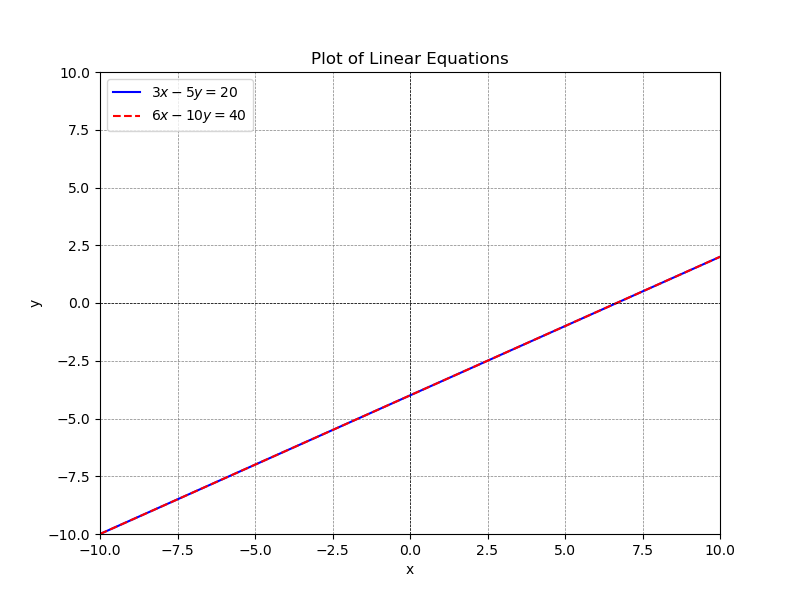
\includegraphics[width=\columnwidth]{figs/lines.png} 
    \label{fig:image_label}
\end{figure}



\end{document}
